% Options for packages loaded elsewhere
\PassOptionsToPackage{unicode}{hyperref}
\PassOptionsToPackage{hyphens}{url}
%
\documentclass[
]{article}
\usepackage{amsmath,amssymb}
\usepackage{iftex}
\ifPDFTeX
  \usepackage[T1]{fontenc}
  \usepackage[utf8]{inputenc}
  \usepackage{textcomp} % provide euro and other symbols
\else % if luatex or xetex
  \usepackage{unicode-math} % this also loads fontspec
  \defaultfontfeatures{Scale=MatchLowercase}
  \defaultfontfeatures[\rmfamily]{Ligatures=TeX,Scale=1}
\fi
\usepackage{lmodern}
\ifPDFTeX\else
  % xetex/luatex font selection
\fi
% Use upquote if available, for straight quotes in verbatim environments
\IfFileExists{upquote.sty}{\usepackage{upquote}}{}
\IfFileExists{microtype.sty}{% use microtype if available
  \usepackage[]{microtype}
  \UseMicrotypeSet[protrusion]{basicmath} % disable protrusion for tt fonts
}{}
\makeatletter
\@ifundefined{KOMAClassName}{% if non-KOMA class
  \IfFileExists{parskip.sty}{%
    \usepackage{parskip}
  }{% else
    \setlength{\parindent}{0pt}
    \setlength{\parskip}{6pt plus 2pt minus 1pt}}
}{% if KOMA class
  \KOMAoptions{parskip=half}}
\makeatother
\usepackage{xcolor}
\usepackage[margin=1in]{geometry}
\usepackage{graphicx}
\makeatletter
\def\maxwidth{\ifdim\Gin@nat@width>\linewidth\linewidth\else\Gin@nat@width\fi}
\def\maxheight{\ifdim\Gin@nat@height>\textheight\textheight\else\Gin@nat@height\fi}
\makeatother
% Scale images if necessary, so that they will not overflow the page
% margins by default, and it is still possible to overwrite the defaults
% using explicit options in \includegraphics[width, height, ...]{}
\setkeys{Gin}{width=\maxwidth,height=\maxheight,keepaspectratio}
% Set default figure placement to htbp
\makeatletter
\def\fps@figure{htbp}
\makeatother
\setlength{\emergencystretch}{3em} % prevent overfull lines
\providecommand{\tightlist}{%
  \setlength{\itemsep}{0pt}\setlength{\parskip}{0pt}}
\setcounter{secnumdepth}{-\maxdimen} % remove section numbering
\usepackage{fullpage}
\usepackage[spanish]{babel}
\usepackage{fancyhdr}
\setlength{\headsep}{7mm}
\usepackage[linktoc=page]{hyperref}
\ifLuaTeX
  \usepackage{selnolig}  % disable illegal ligatures
\fi
\IfFileExists{bookmark.sty}{\usepackage{bookmark}}{\usepackage{hyperref}}
\IfFileExists{xurl.sty}{\usepackage{xurl}}{} % add URL line breaks if available
\urlstyle{same}
\hypersetup{
  hidelinks,
  pdfcreator={LaTeX via pandoc}}

\author{}
\date{\vspace{-2.5em}}

\begin{document}

\setlength{\headheight}{13.6pt}
\setlength{\topmargin}{-10mm}

\rhead{Minería de Datos}
\lhead{Entrega D3}

\pagestyle{fancy}

\cfoot{\thepage}
\setcounter{page}{149}

\#Anexo

\hypertarget{profiling-fuzzy}{%
\subsection{Profiling Fuzzy}\label{profiling-fuzzy}}

\begin{figure}
\includegraphics[width=0.75\linewidth,height=0.75\textheight]{Anexo_files/figure-latex/unnamed-chunk-5-1} \caption{Medias de la Edad en años del coche del cliente por clúster respecto la media global}\label{fig:unnamed-chunk-5}
\end{figure}

\begin{figure}
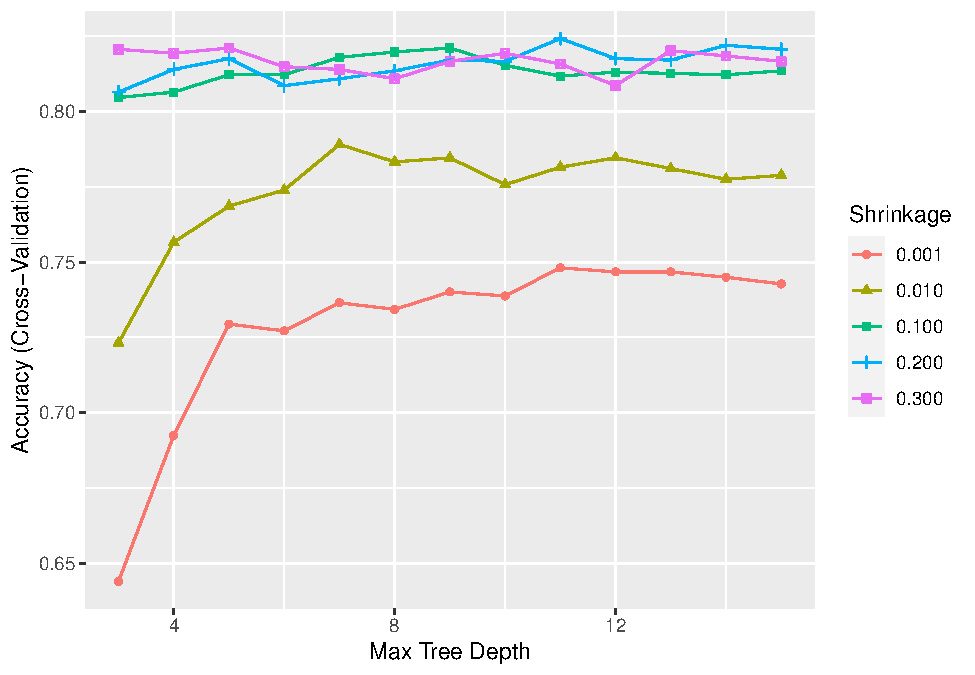
\includegraphics[width=0.75\linewidth,height=0.75\textheight]{Anexo_files/figure-latex/unnamed-chunk-6-1} \caption{Medias del Número de familiares del cliente por clúster respecto la media global}\label{fig:unnamed-chunk-6}
\end{figure}

\begin{figure}
\includegraphics[width=0.75\linewidth,height=0.75\textheight]{Anexo_files/figure-latex/unnamed-chunk-7-1} \caption{Medias del logaritmo de los Ingresos totales del cliente por clúster respecto la media global}\label{fig:unnamed-chunk-7}
\end{figure}

\begin{figure}
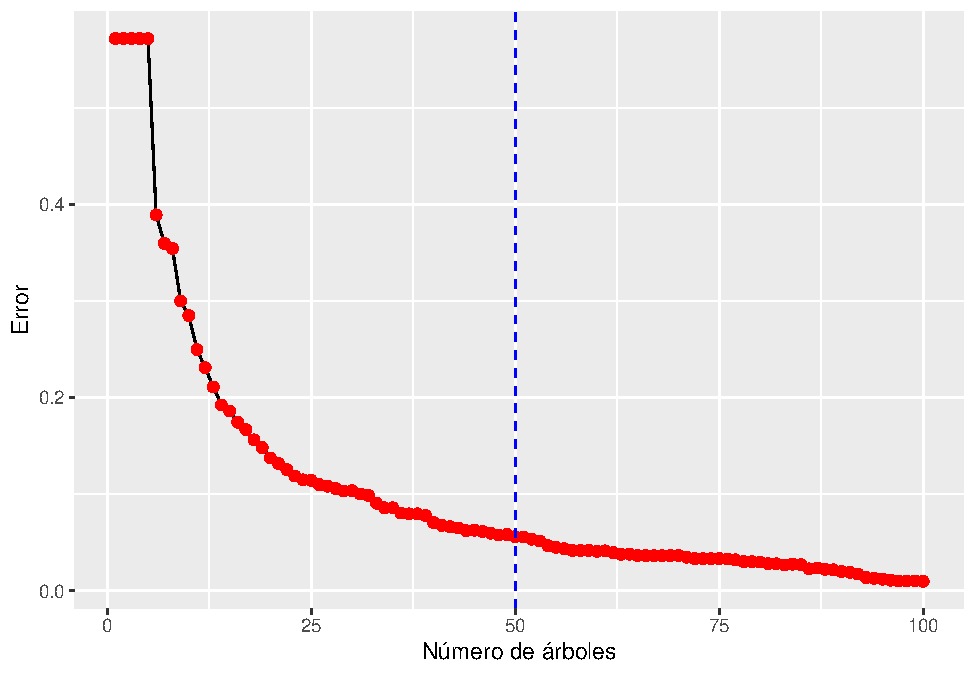
\includegraphics[width=0.75\linewidth,height=0.75\textheight]{Anexo_files/figure-latex/unnamed-chunk-8-1} \caption{Medias del Importe de crédito del préstamo por clúster respecto la media global}\label{fig:unnamed-chunk-8}
\end{figure}

\begin{figure}
\includegraphics[width=0.75\linewidth,height=0.75\textheight]{Anexo_files/figure-latex/unnamed-chunk-9-1} \caption{Medias de la Edad por clúster respecto la media global}\label{fig:unnamed-chunk-9}
\end{figure}

\begin{figure}
\includegraphics[width=0.75\linewidth,height=0.75\textheight]{Anexo_files/figure-latex/unnamed-chunk-10-1} \caption{Gráfico de la distribución del Género respecto el Clúster}\label{fig:unnamed-chunk-10}
\end{figure}

\begin{figure}
\includegraphics[width=0.75\linewidth,height=0.75\textheight]{Anexo_files/figure-latex/unnamed-chunk-11-1} \caption{Gráfico de la distribución del Tipo de ingresos respecto el Clúster}\label{fig:unnamed-chunk-11}
\end{figure}

\begin{figure}
\includegraphics[width=0.75\linewidth,height=0.75\textheight]{Anexo_files/figure-latex/unnamed-chunk-12-1} \caption{Gráfico de la distribución del Nivel de estudios del cliente respecto el Clúster}\label{fig:unnamed-chunk-12}
\end{figure}

\begin{figure}
\includegraphics[width=0.75\linewidth,height=0.75\textheight]{Anexo_files/figure-latex/unnamed-chunk-13-1} \caption{Gráfico de la distribución del Estado civil respecto el Clúster}\label{fig:unnamed-chunk-13}
\end{figure}

\begin{figure}
\includegraphics[width=0.75\linewidth,height=0.75\textheight]{Anexo_files/figure-latex/unnamed-chunk-14-1} \caption{Gráfico de la distribución de la Actividad laboral respecto el Clúster}\label{fig:unnamed-chunk-14}
\end{figure}

\begin{figure}
\includegraphics[width=0.75\linewidth,height=0.75\textheight]{Anexo_files/figure-latex/unnamed-chunk-15-1} \caption{Gráfico de la distribución del Tipo de organización donde trabaja el cliente respecto el Clúster}\label{fig:unnamed-chunk-15}
\end{figure}

\begin{figure}
\includegraphics[width=0.75\linewidth,height=0.75\textheight]{Anexo_files/figure-latex/unnamed-chunk-16-1} \caption{Gráfico de la distribución de la Calificación de la región donde vive el cliente}\label{fig:unnamed-chunk-16}
\end{figure}

\hypertarget{profiling-k-means}{%
\subsection{Profiling k-means}\label{profiling-k-means}}

\begin{figure}
\includegraphics[width=0.75\linewidth,height=0.75\textheight]{Anexo_files/figure-latex/unnamed-chunk-21-1} \caption{Medias del Número de familiares del cliente por clúster respecto la media global}\label{fig:unnamed-chunk-21}
\end{figure}

\begin{figure}
\includegraphics[width=0.75\linewidth,height=0.75\textheight]{Anexo_files/figure-latex/unnamed-chunk-22-1} \caption{Medias del logaritmo de los Ingresos totales del cliente por clúster respecto la media global}\label{fig:unnamed-chunk-22}
\end{figure}

\begin{figure}
\includegraphics[width=0.75\linewidth,height=0.75\textheight]{Anexo_files/figure-latex/unnamed-chunk-23-1} \caption{Medias del Importe de crédito del préstamo por clúster respecto la media global}\label{fig:unnamed-chunk-23}
\end{figure}

\begin{figure}
\includegraphics[width=0.75\linewidth,height=0.75\textheight]{Anexo_files/figure-latex/unnamed-chunk-24-1} \caption{Medias de la Edad por clúster respecto la media global}\label{fig:unnamed-chunk-24}
\end{figure}

\begin{figure}
\includegraphics[width=0.75\linewidth,height=0.75\textheight]{Anexo_files/figure-latex/unnamed-chunk-25-1} \caption{Gráfico de la distribución del Género respecto el Clúster}\label{fig:unnamed-chunk-25}
\end{figure}

\begin{figure}
\includegraphics[width=0.75\linewidth,height=0.75\textheight]{Anexo_files/figure-latex/unnamed-chunk-26-1} \caption{Gráfico de la distribución del Tipo de ingresos respecto el Clúster}\label{fig:unnamed-chunk-26}
\end{figure}

\begin{figure}
\includegraphics[width=0.75\linewidth,height=0.75\textheight]{Anexo_files/figure-latex/unnamed-chunk-27-1} \caption{Gráfico de la distribución del Nivel de estudios del cliente respecto el Clúster}\label{fig:unnamed-chunk-27}
\end{figure}

\begin{figure}
\includegraphics[width=0.75\linewidth,height=0.75\textheight]{Anexo_files/figure-latex/unnamed-chunk-28-1} \caption{Gráfico de la distribución del Estado civil respecto el Clúster}\label{fig:unnamed-chunk-28}
\end{figure}

\begin{figure}
\includegraphics[width=0.75\linewidth,height=0.75\textheight]{Anexo_files/figure-latex/unnamed-chunk-29-1} \caption{Gráfico de la distribución de la Actividad laboral respecto el Clúster}\label{fig:unnamed-chunk-29}
\end{figure}

\begin{figure}
\includegraphics[width=0.75\linewidth,height=0.75\textheight]{Anexo_files/figure-latex/unnamed-chunk-30-1} \caption{Gráfico de la distribución del Tipo de organización donde trabaja el cliente respecto el Clúster}\label{fig:unnamed-chunk-30}
\end{figure}

\begin{figure}
\includegraphics[width=0.75\linewidth,height=0.75\textheight]{Anexo_files/figure-latex/unnamed-chunk-31-1} \caption{Gráfico de la distribución de la Calificación de la región donde vive el cliente respecto el Clúster}\label{fig:unnamed-chunk-31}
\end{figure}

\hypertarget{profiling-cure}{%
\subsection{Profiling CURE}\label{profiling-cure}}

\textbf{Variables numéricas}

\begin{figure}
\includegraphics[width=0.75\linewidth,height=0.75\textheight]{Anexo_files/figure-latex/unnamed-chunk-34-1} \caption{Comparación de medias por cluster OWN CAR AGE}\label{fig:unnamed-chunk-34}
\end{figure}

\begin{figure}
\includegraphics[width=0.75\linewidth,height=0.75\textheight]{Anexo_files/figure-latex/unnamed-chunk-35-1} \caption{Comparación de medias por cluster CNT FAM MEMBERS}\label{fig:unnamed-chunk-35}
\end{figure}

\begin{figure}
\includegraphics[width=0.75\linewidth,height=0.75\textheight]{Anexo_files/figure-latex/unnamed-chunk-36-1} \caption{Comparación de medias por LOG AMT INCOME TOTAL}\label{fig:unnamed-chunk-36}
\end{figure}

\begin{figure}
\includegraphics[width=0.75\linewidth,height=0.75\textheight]{Anexo_files/figure-latex/unnamed-chunk-37-1} \caption{Comparación de medias por LOG AMT CREDIT}\label{fig:unnamed-chunk-37}
\end{figure}

\begin{figure}
\includegraphics[width=0.75\linewidth,height=0.75\textheight]{Anexo_files/figure-latex/unnamed-chunk-38-1} \caption{Comparación de medias por cluster AGE YEARS}\label{fig:unnamed-chunk-38}
\end{figure}

\begin{figure}
\includegraphics[width=0.75\linewidth,height=0.75\textheight]{Anexo_files/figure-latex/unnamed-chunk-39-1} \caption{Comparación de medias por cluster RATIO CREDIT INCOME}\label{fig:unnamed-chunk-39}
\end{figure}

\begin{figure}
\includegraphics[width=0.75\linewidth,height=0.75\textheight]{Anexo_files/figure-latex/unnamed-chunk-40-1} \caption{Comparación de medias por cluster RATIO ANNUITY CREDIT}\label{fig:unnamed-chunk-40}
\end{figure}

\begin{figure}
\includegraphics[width=0.75\linewidth,height=0.75\textheight]{Anexo_files/figure-latex/unnamed-chunk-41-1} \caption{Comparación de medias por cluster DTI RATIO}\label{fig:unnamed-chunk-41}
\end{figure}

\textbf{Variables categóricas}

\begin{figure}
\includegraphics[width=0.75\linewidth,height=0.75\textheight]{Anexo_files/figure-latex/unnamed-chunk-42-1} \caption{Comparación de proporción por cluster CODE GENDER}\label{fig:unnamed-chunk-42}
\end{figure}

\begin{figure}
\includegraphics[width=0.75\linewidth,height=0.75\textheight]{Anexo_files/figure-latex/unnamed-chunk-43-1} \caption{Comparación de proporción por cluster NAME INCOME TYPE}\label{fig:unnamed-chunk-43}
\end{figure}

\includegraphics{Anexo_files/figure-latex/unnamed-chunk-44-1.pdf}

\begin{figure}
\includegraphics[width=0.75\linewidth,height=0.75\textheight]{Anexo_files/figure-latex/unnamed-chunk-45-1} \caption{Comparación de proporción por cluster NAME FAMILY STATUS}\label{fig:unnamed-chunk-45}
\end{figure}

\begin{figure}
\includegraphics[width=0.75\linewidth,height=0.75\textheight]{Anexo_files/figure-latex/unnamed-chunk-46-1} \caption{Comparación de proporción por cluster OCCUPATION TYPE}\label{fig:unnamed-chunk-46}
\end{figure}

\begin{figure}
\includegraphics[width=0.75\linewidth,height=0.75\textheight]{Anexo_files/figure-latex/unnamed-chunk-47-1} \caption{Comparación de proporción por cluster ORGANIZATION TYPE}\label{fig:unnamed-chunk-47}
\end{figure}

\begin{figure}
\includegraphics[width=0.75\linewidth,height=0.75\textheight]{Anexo_files/figure-latex/unnamed-chunk-48-1} \caption{Comparación de proporción por cluster REGION RATING CLIENT}\label{fig:unnamed-chunk-48}
\end{figure}

\end{document}
